\begin{figure}
\begin{center}
    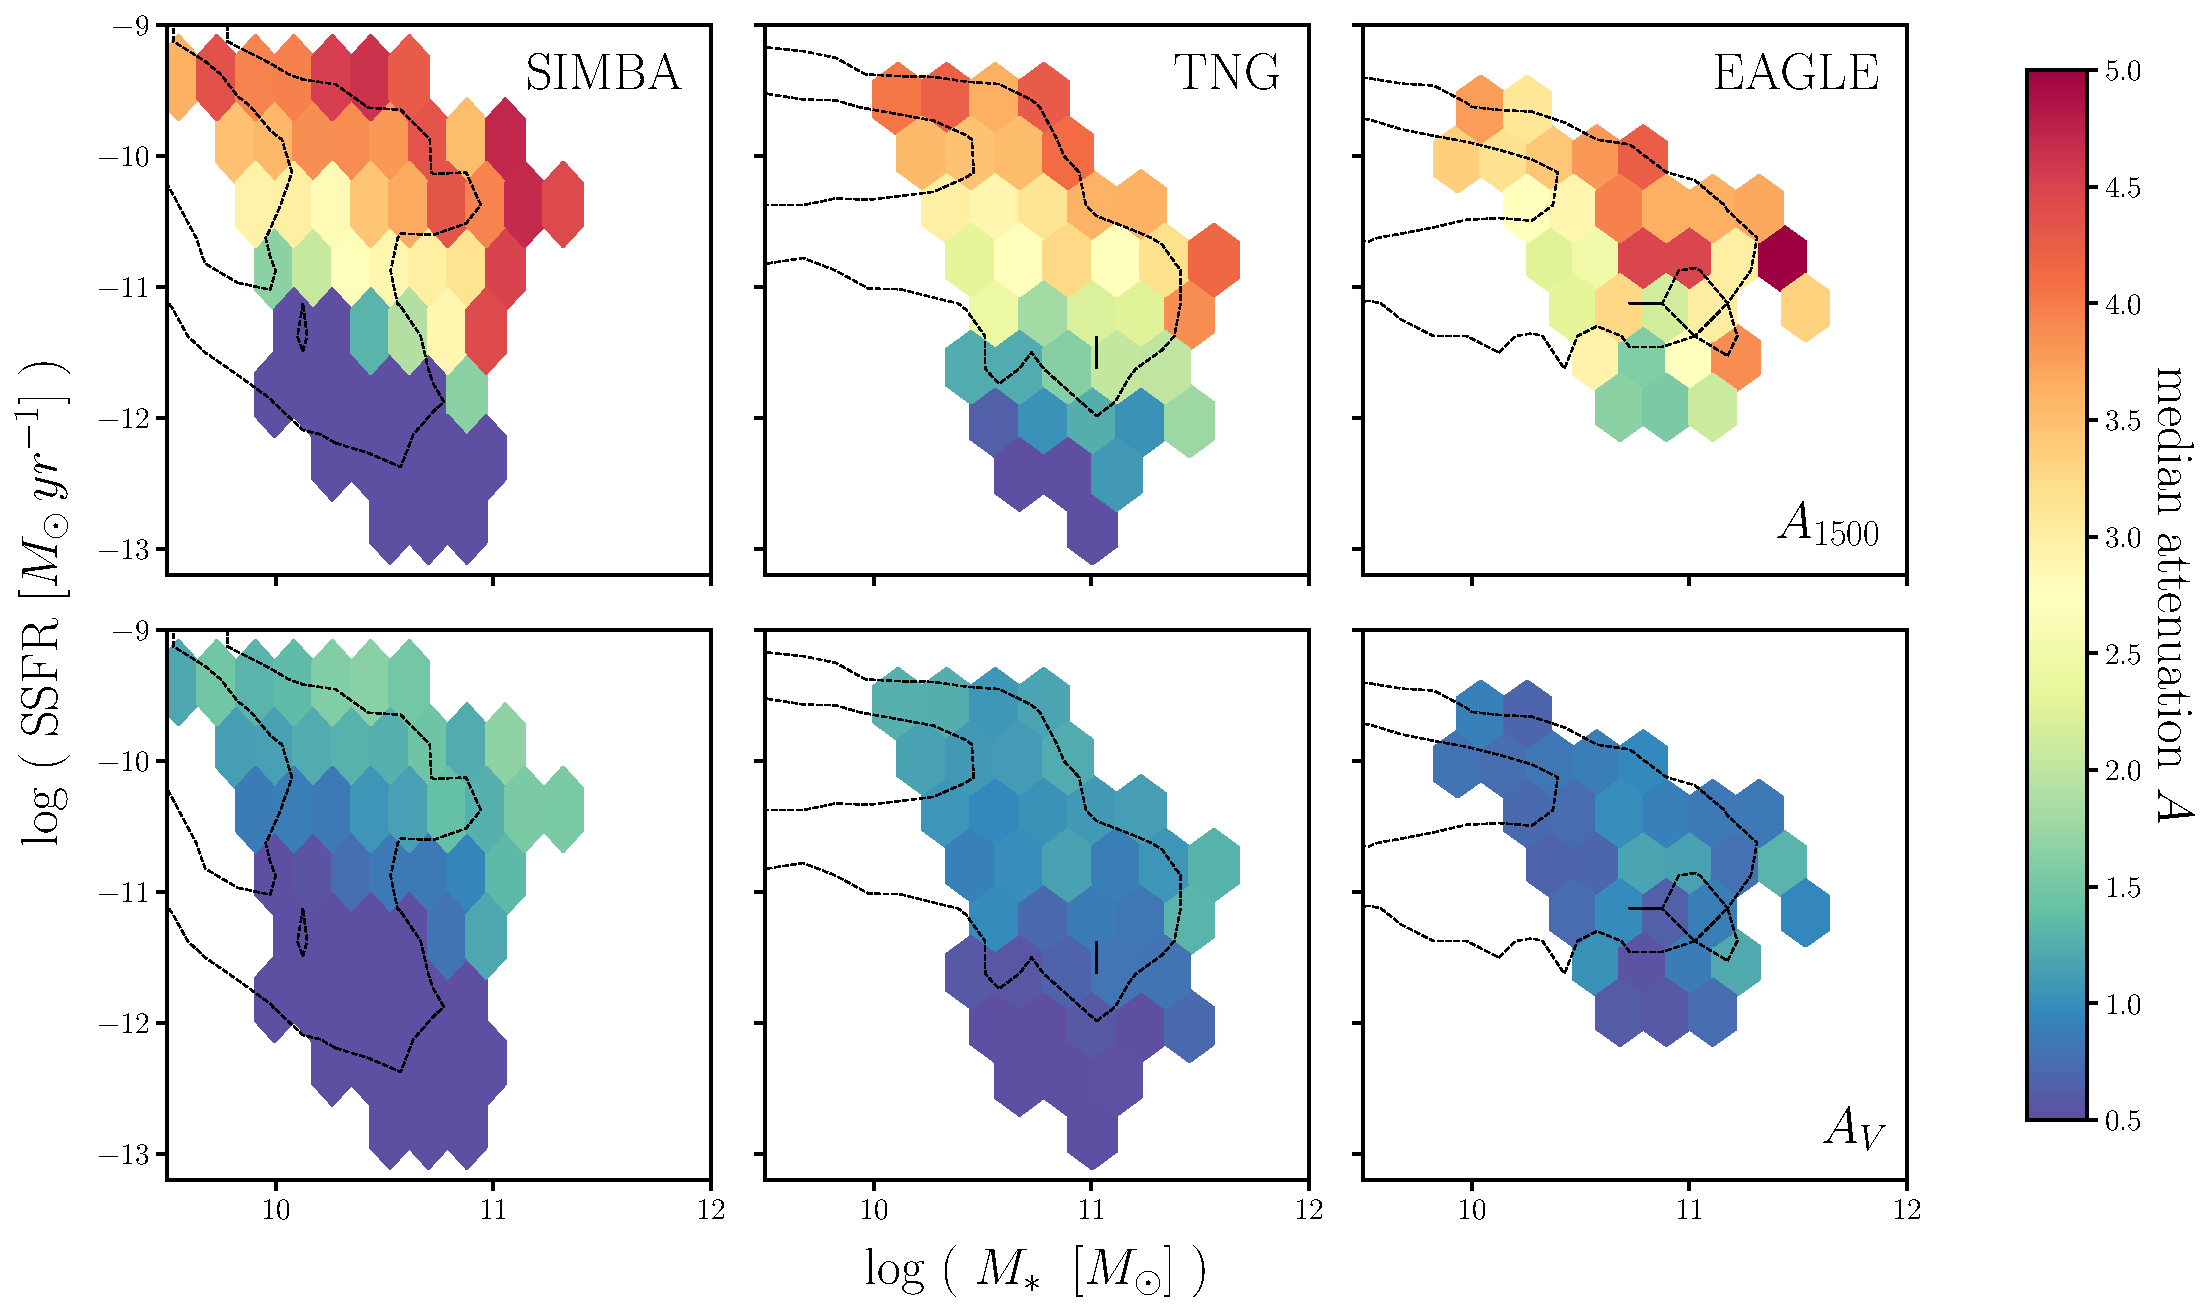
\includegraphics[width=0.9\textwidth]{figs/abc_av_mssfr.pdf}
    \caption{\label{fig:avmsfr}
    \chedit{ 
        $M_*$ and $\ssfr$ dependence of dust attenuation at $1500 \AA$
        ($A_{1500}$; top) and at $5500\AA$ ($A_{V}$ bottom) predicted by the
        \eda~for TNG (left) and EAGLE (right). The colormap in each hexbin 
        represents the median attenuation for all simulated galaxies in the
        bin (right color bar). We only include bins with more than 10 galaxies that
        satisfy our $M_r < -20$ completeness limit.
        For reference, we include in each panel the $M_*-\ssfr$ relation of
        all galaxies from the simulations (black dashed).
        Overall, TNG and EAGLE galaxies with higher $M_*$ have higher dust
        attenuation --- consistent with the literature.
        Furthermore, since previous works have primarily focused on star-forming
        galaxies, the \eda~provides new insight into the $\ssfr$ dependence of
        dust attenuation: simulated galaxies with higher $\ssfr$ have steeper
        attenuation curves. 
    }
    }
\end{center}
\end{figure}

\subsection{The Galaxy -- Dust Connection}  
With the \eda~framework, we can also shed light on the connection between
the physical properties of the simulated galaxies and dust attenuations.
In our \eda~prescription, we included a flexible $M_*$ and $\ssfr$ dependence in both the
amplitude and slope of the attenuation curve~(Eqs~\ref{eq:tauv}
and~\ref{eq:delta}). 
Hence, we can reveal the $M_*$ and $\ssfr$ dependence of dust attenuation
through both the \eda~parameter constraints (Figure~\ref{fig:abc}) and the
predicted attenuation curves. 

%           $m_{\tau,M_*}$,$m_{\tau,{\rm SSFR}}$,$c_{\tau}$,$m_{\delta,M_*}$,$m_{\delta,{\rm SSFR}}$,$c_\delta$
%SIMBA:     1.27 +0.46 -0.46	1.28 +0.24 -0.23	1.58 +0.12 -0.12	0.07 +0.12 -0.11	0.13 +0.10 -0.10	-0.18 +0.04 -0.04
%TNG:       0.57 +0.44 -0.53	0.62 +0.21 -0.20	1.34 +0.19 -0.21	-0.18 +0.20 -0.19	-0.19 +0.15 -0.16	-0.07 +0.08 -0.08
%EAGLE:     0.59 +0.33 -0.33	0.18 +0.20 -0.17	0.81 +0.14 -0.15	-0.13 +0.17 -0.18	-0.22 +0.14 -0.14	-0.34 +0.08 -0.08

%%%%%%%%%%%%%%%%%%%%%%%%%%%%%%%%%%%%%%%%%%
% table of free parameters
%%%%%%%%%%%%%%%%%%%%%%%%%%%%%%%%%%%%%%%%%%
\begin{table}
    \caption{Inferred the Empirical Dust Attenuation Model Parameters}
    \begin{tabular}{lcccccc} \toprule
        & $m_{\tau,M_*}$ & $m_{\tau,\ssfr}$ & $c_\tau$ & $m_{\delta,M_*}$ & $m_{\delta,\ssfr}$ & $c_\delta$ \\[3pt] \hline\hline
        SIMBA   & $1.27\substack{+0.46\\-0.46}$ &
        $1.28\substack{+0.24\\-0.23}$ & $1.58\substack{+0.12\\-0.12}$ &
        $0.07 \substack{+0.12\\-0.11}$ & $0.13 \substack{+0.10\\-0.10}$ &
        $-0.18\substack{+0.04\\-0.04}$ \\
        TNG     & $0.57\substack{+0.44\\-0.53}$ &
        $0.62\substack{+0.21\\-0.20}$ & $1.34\substack{+0.19\\-0.21}$ &
        $-0.18\substack{+0.20\\-0.19}$ & $-0.19\substack{+0.15\\-0.16}$ &
        $-0.07\substack{+0.08\\-0.08}$ \\
        EAGLE   & $0.59\substack{+0.33\\-0.33}$ &
        $0.18\substack{+0.20\\-0.17}$ & $0.81\substack{+0.14\\-0.15}$ &
        $-0.13\substack{+0.17\\-0.18}$ & $-0.22\substack{+0.14\\-0.14}$ &
        $-0.34\substack{+0.08\\-0.08}$\\
        \hline
    \end{tabular} \label{tab:posterior}
\end{table}

\chedit{
    In the last section, we discussed the $\ssfr$ dependence of the \eda~attenuation
    curves: quiescent galaxies have attenuation curves with shallower slopes
    and lower amplitude than star-forming galaxies. 
    We now focus on the $M_*$ dependence of dust attenuation. 
    In Table~\ref{tab:posterior}, we list the median values and the 68\%
    confidence interval of the inferred \eda~parameter posteriors for the 
    three simulations. 
    In SIMBA, TNG, and EAGLE, we find significant $M_*$ dependence in
    $\tau_V$: $V$-band dust attenuation is higher for more massive galaxies.  
    Meanwhile, we find little $M_*$ dependence in the slope of the dust
    attenuation.
}

We take a closer look at the $M_*$ and $\ssfr$ dependence of the
attenuation curve in Figure~\ref{fig:avmsfr}. 
We present dust attenuation at $1500\AA$ ($A_{1500}$; top) and $5500\AA$
($A_V$; bottom) as a function of $\log M_*$ and $\log \ssfr$ predicted by the
\eda~for SIMBA (left), TNG (center) and EAGLE (right). 
For each hexbin, the colormap represents the median attenuation for all
simulated galaxies in the bin. 
We only include bins with more than 10 galaxies that satisfy our selection
function. 
We include, for reference, the $M_* - \ssfr$ relation of the simulations in
black dashed contours.

In each panel, we find that SIMBA, TNG, and EAGLE galaxies with higher
$M_*$ have higher dust attenuation --- consistent with the literature.
\cite{burgarella2005}, for instance, found significant positive $M_*$
dependence in $FUV$ attenuation in NUV-selected and FIR-selected samples. 
\cite{garn2010} and \cite{battisti2016} also find higher attenuation in
more massive SDSS star-forming galaxies. 
Most recently, \cite{salim2018} find higher $V$ and $FUV$ attenuation for
more massive star-forming galaxies in GSWLC2. 
\chedit{ 
    For the $\ssfr$ dependence, we find that galaxies with higher $\ssfr$ have
    higher $A_{1500}$ (top) and $A_V$ (bottom). 
    Furthermore, galaxies with higher $\ssfr$ have steeper slopes; quiescent
    galaxies with the lowest $\ssfr$  have nearly flat attenuation curves. 
    Since observations have only focused on star-forming galaxies due to the
    difficulty in measuring dust attenuation in quiescent galaxies, the
    \eda~predictions provide new insight into the $\ssfr$ dependence of dust attenuation. 
    In summary, from the \eda~predictions, we find that \emph{SIMBA, TNG, and
    EAGLE galaxies with higher $M_*$ require overall higher dust attenuation
    and galaxies with higher $\ssfr$ require steeper attenuation curves}.
} 
